\subsection{Distrución del uso de las estaciones}

En la figura \ref{fig:map_metro_stations} se visualiza las linea del metro y del metrobus. Como se mencionó en la introduccion, el sistema público de bicicletas está enfocado en disminuir la congestión del tráfico usando vías adecuadas y en puntos apropiados. Esto se ve reflejado en las estaciones de MiBici, esto es debido a que la mayoria se encuentra en los poligonos de intervencion urbana especial (PIUE), las cuales son áreas enfocadas al desarrollo social, medioambiental y económico\cite{poligono_2018}. Aunado a esto, las estaciones que estan fuera de estos polígonos, se encuentran alrededor de las lineas del metro. Esto puede ser debido a que fueron instaladas para suplir el uso del metro cuando no sea eficiente para el usuario.

\begin{figure}[H]
    \centering
    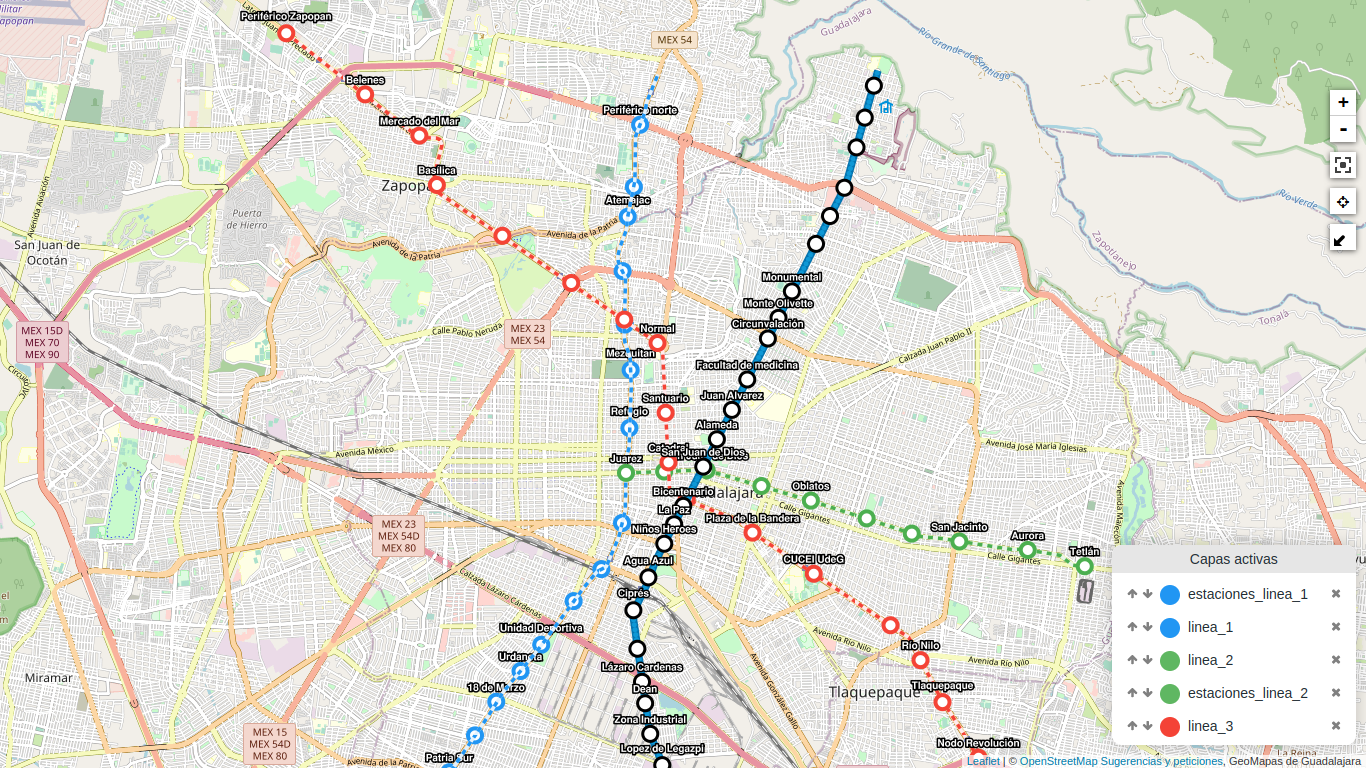
\includegraphics[width=8cm,height=5cm]{Graphics/map_with_metro_lines.png}
    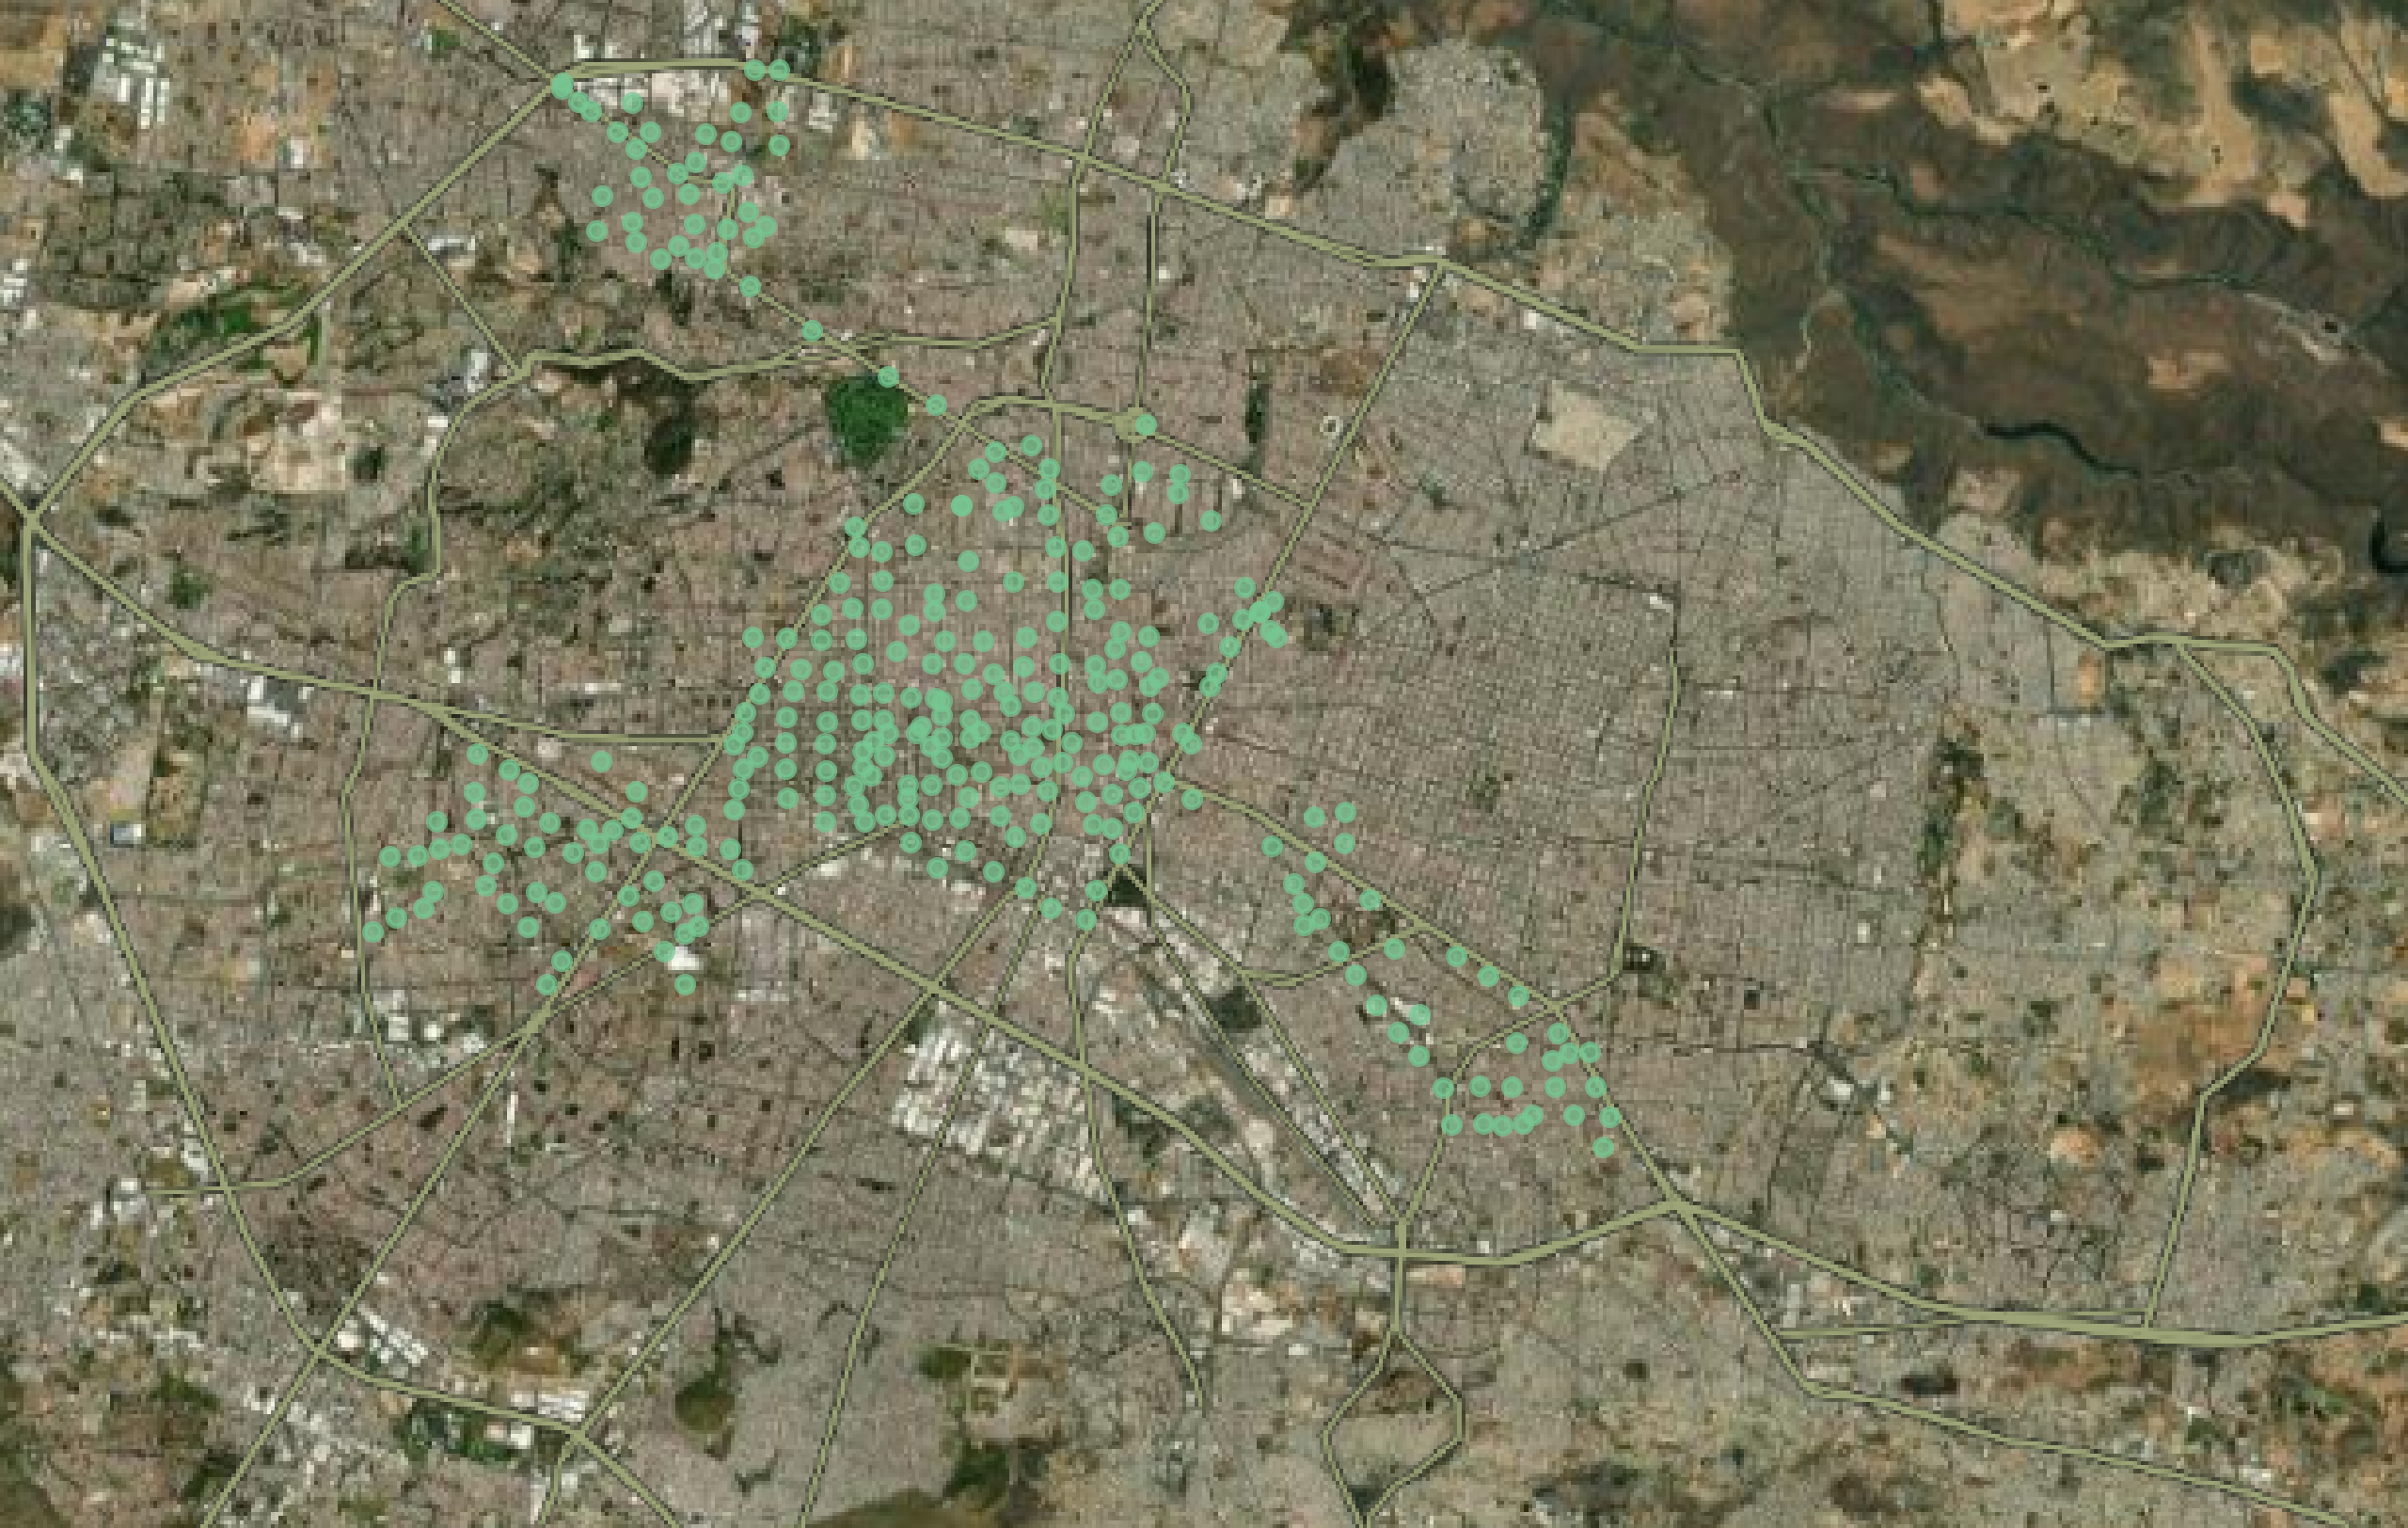
\includegraphics[width=8cm,height=5cm]{Graphics/stations.png}
    \caption{Mapa de la zona metropolitana de Guadalajara señalando las lineas del metro (izquierda) y las estaciones de MiBici (derecha).}
    \label{fig:map_metro_stations}
\end{figure}

En la figura \ref{fig:distribution_station_all_origin} se puede notar como las estaciones localizadas en los PIUE son las más usadas con respecto a las estaciones que se encuentran en las orillas de la zona metropolitana. En la figura \ref{fig:distribution_station_zoom_origin} se visualiza que las estaciones que se encuentran sobre la Avenida Ignación L. Vallarta y las que se encuentran en las intersecciones de las lineas de metro.

\begin{figure}[H]
    \centering
    \begin{subfigure}[b]{8cm}
        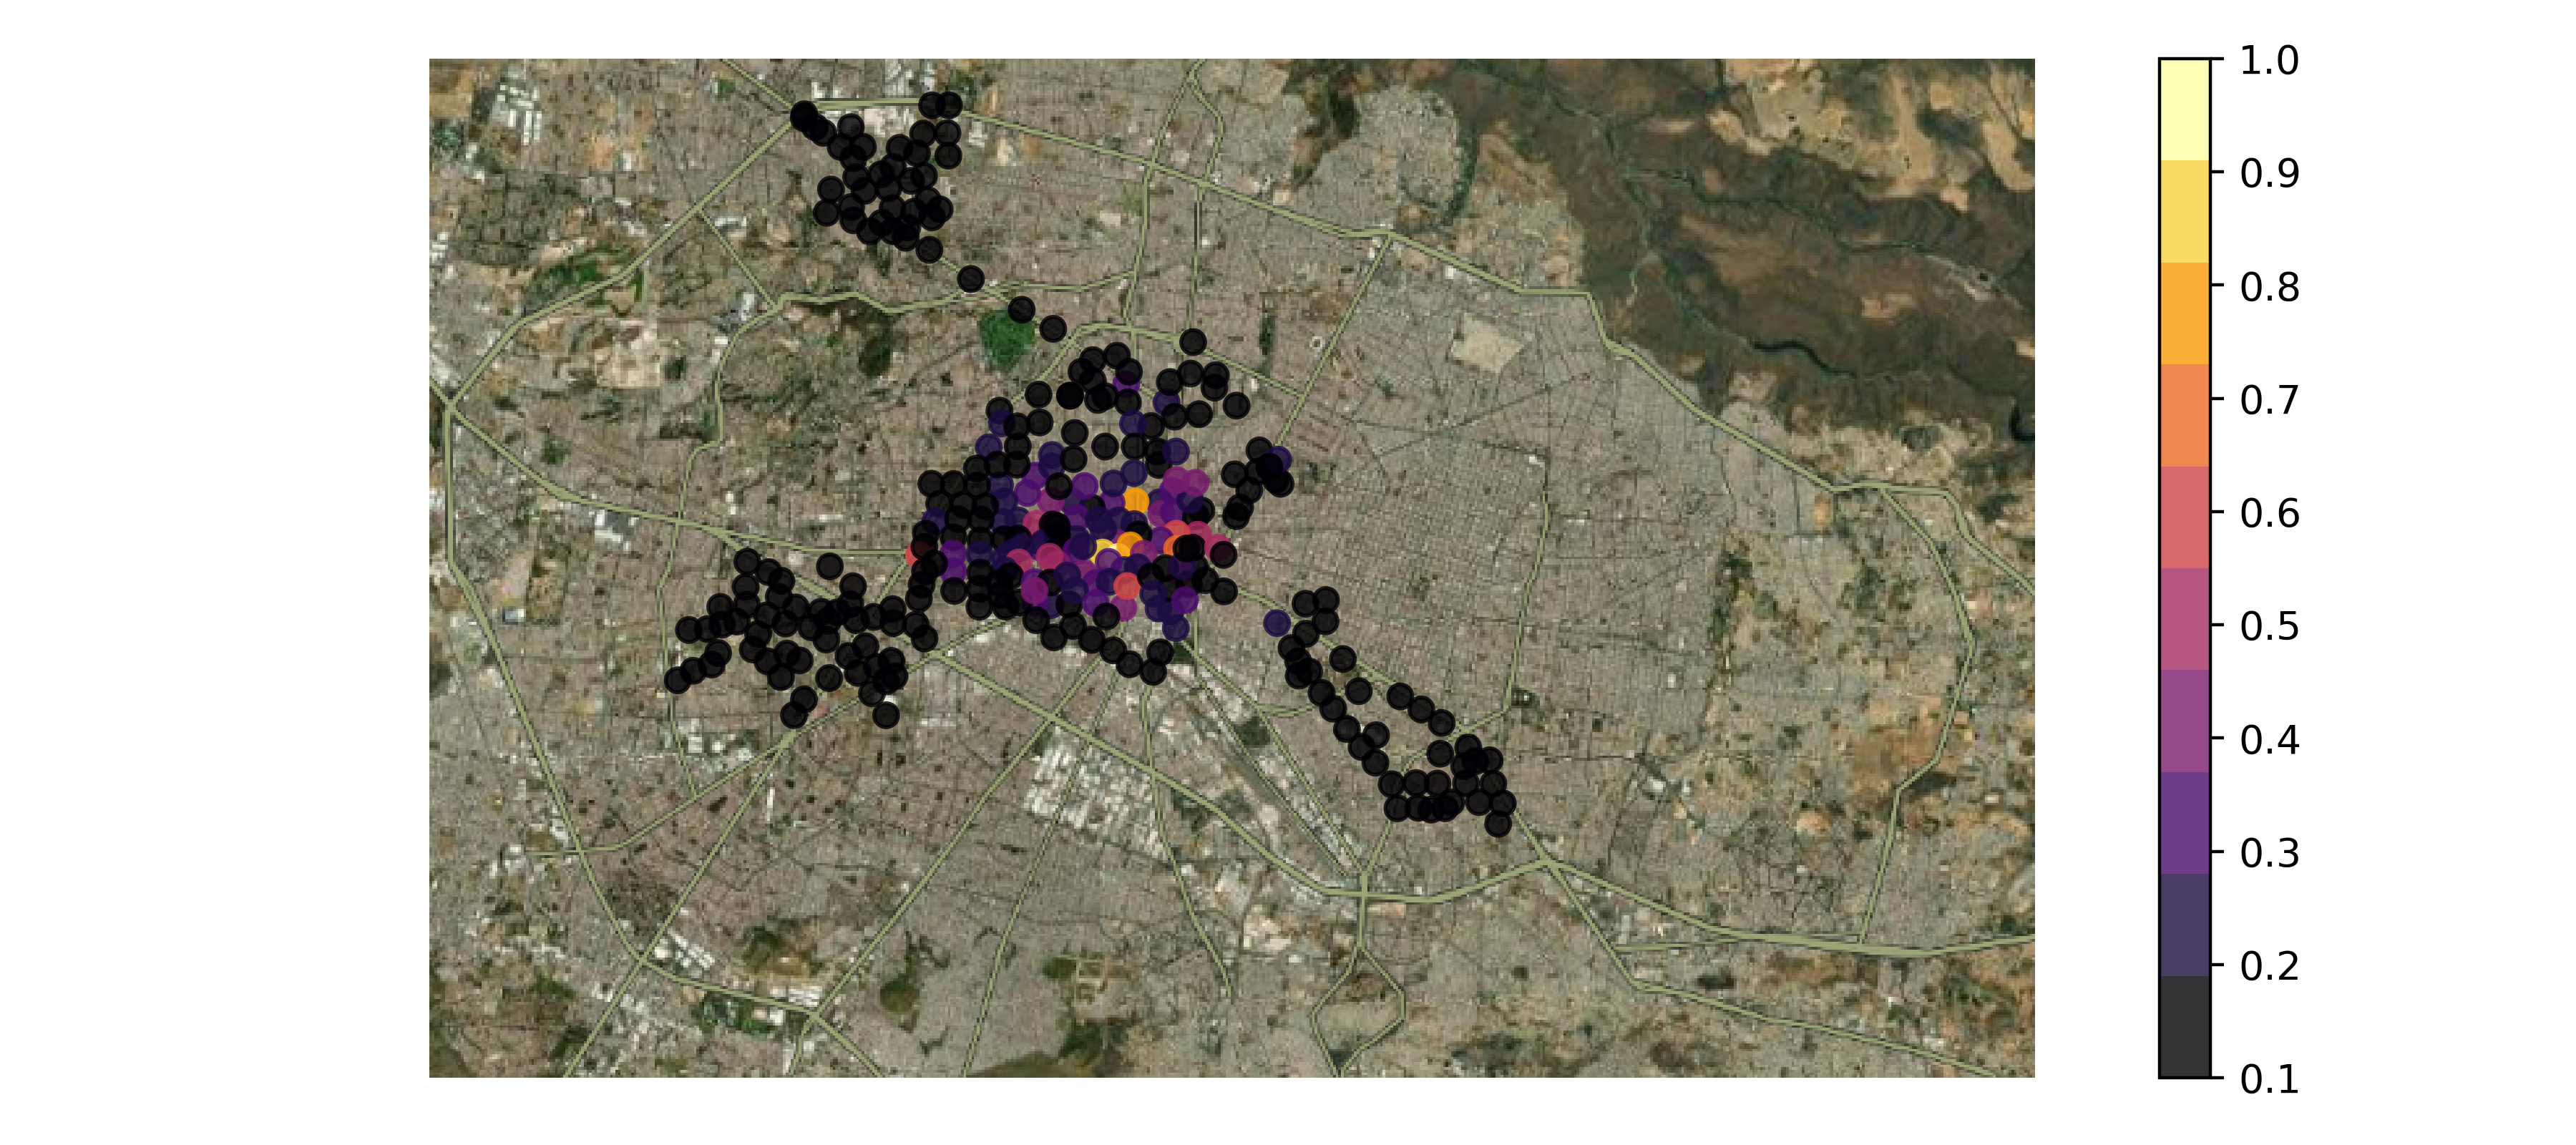
\includegraphics[width=8cm]{Graphics/repetition_origen.png}
        \caption{Zona metropolitana de Guadalajara.}
        \label{fig:distribution_station_all_origin}
    \end{subfigure}
    \hspace{0.5cm}
    \begin{subfigure}[b]{8cm}
        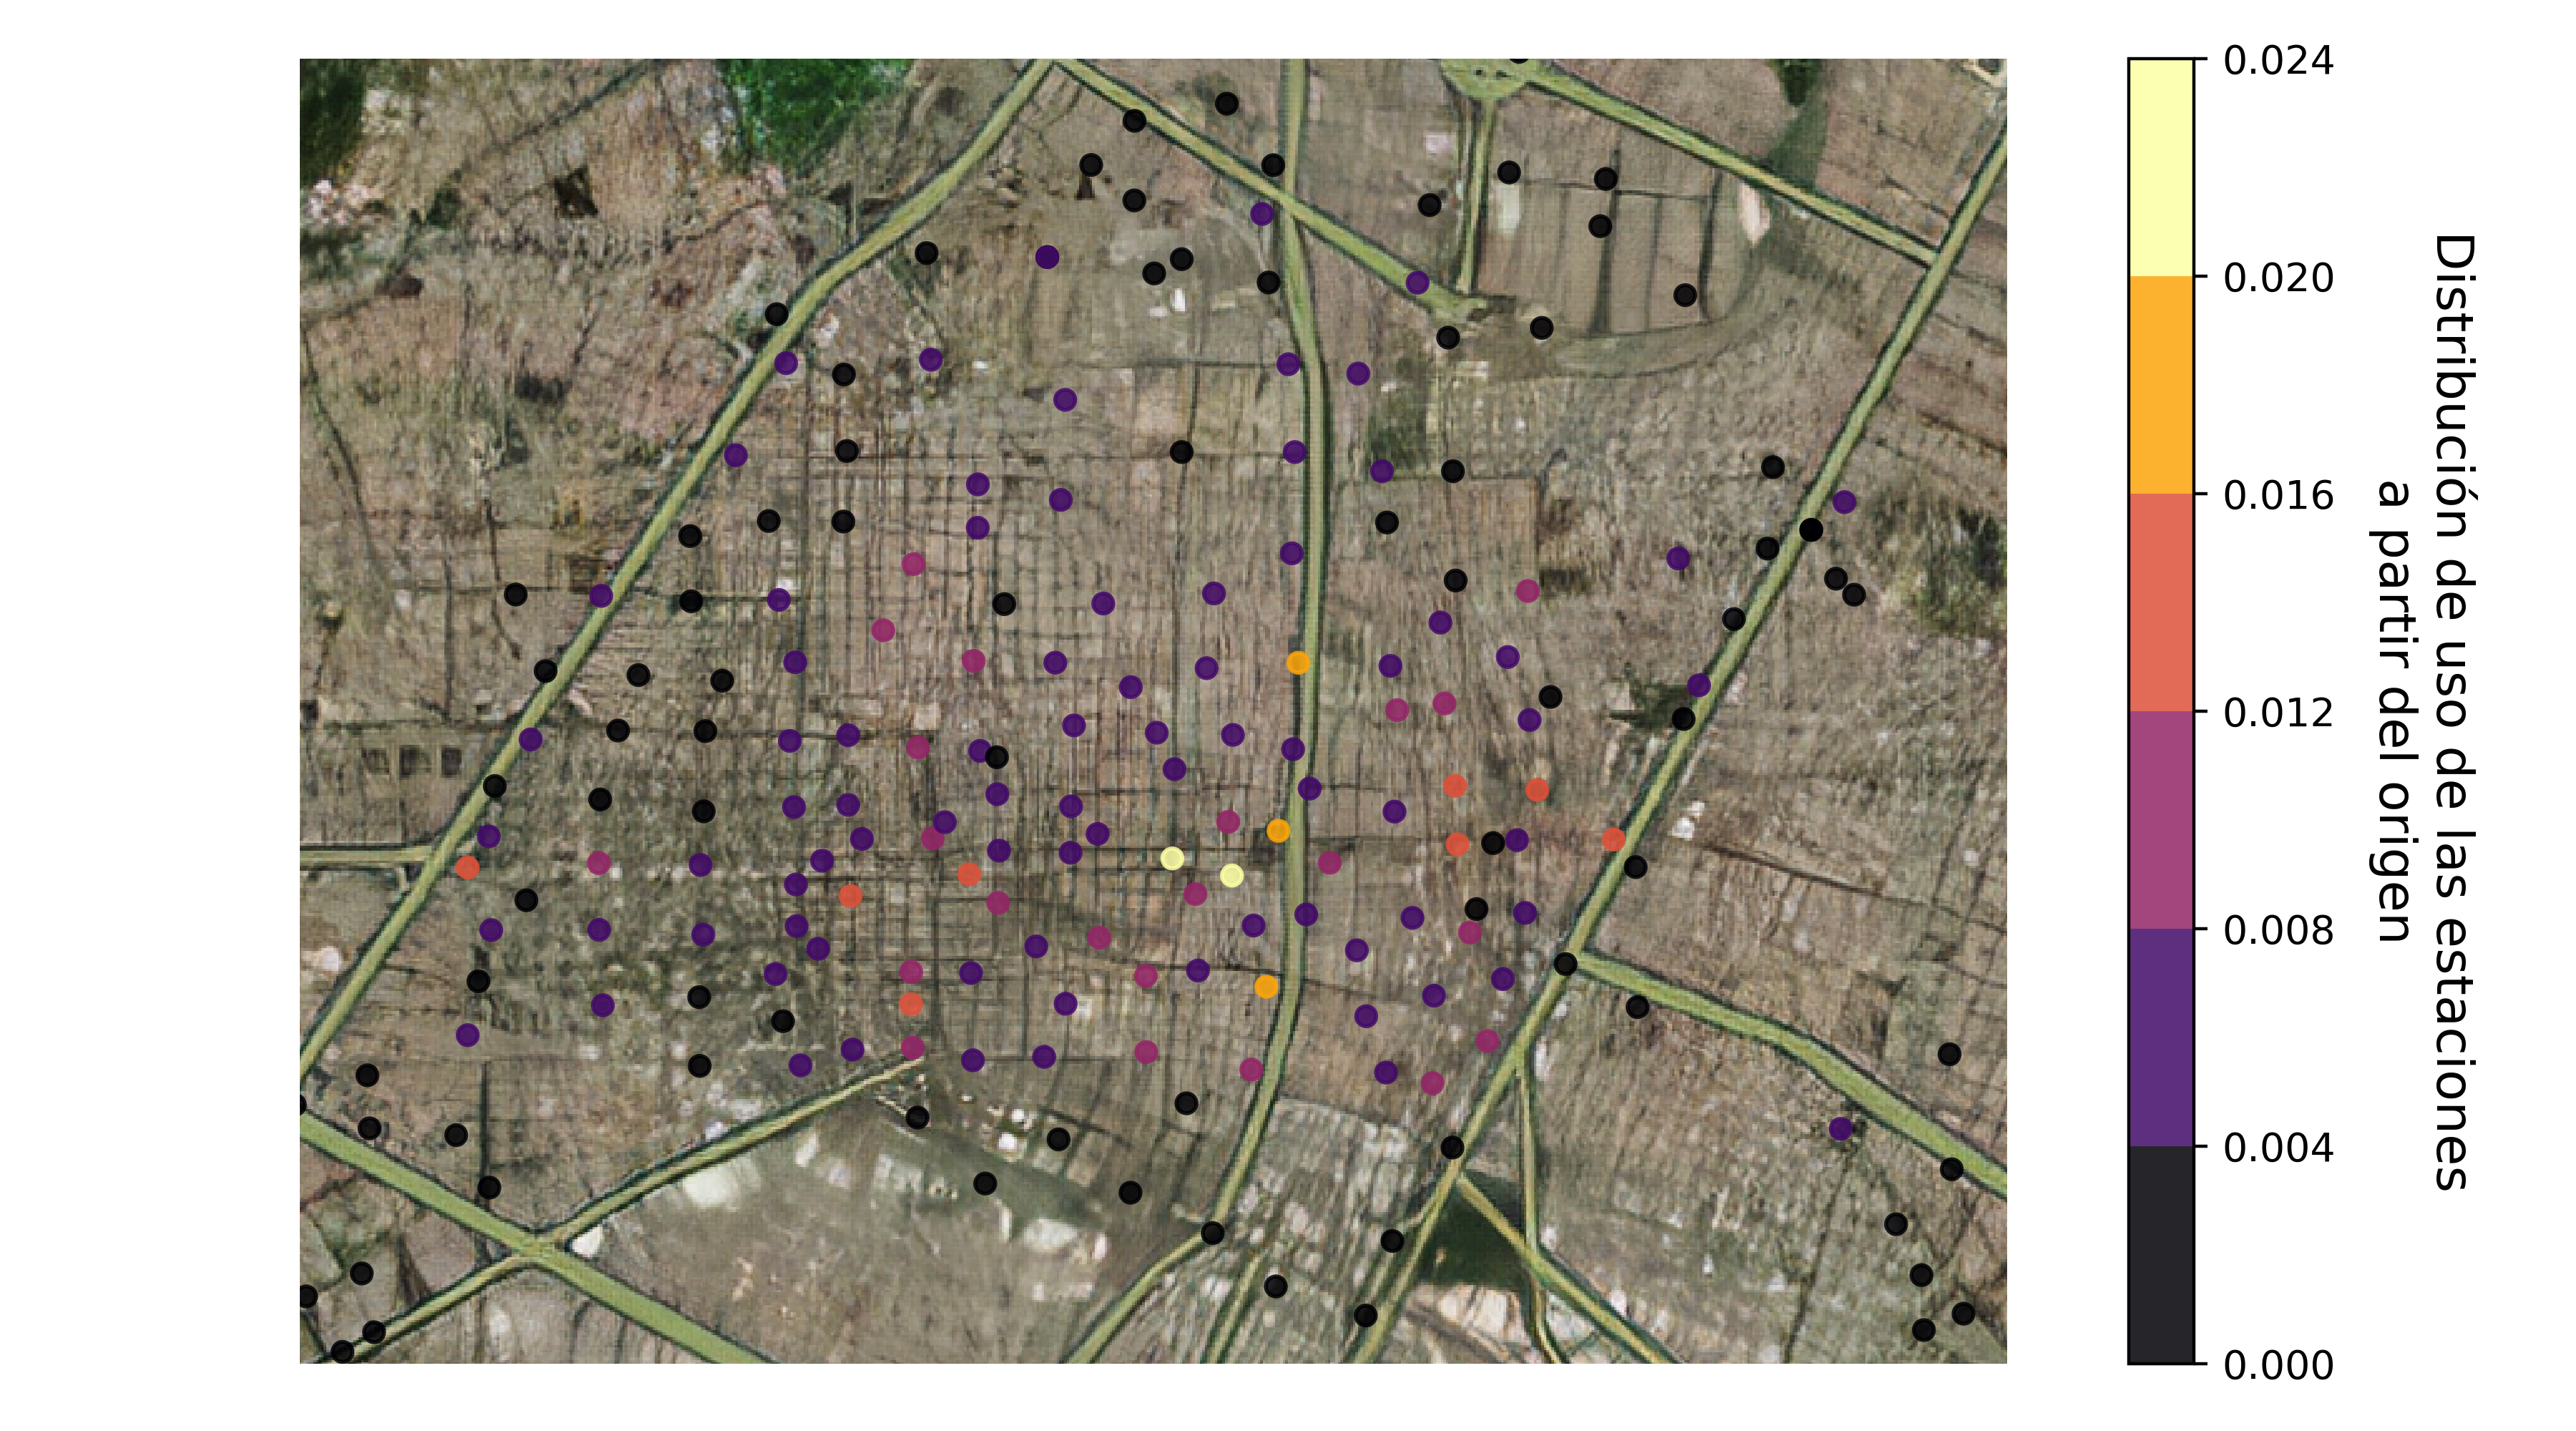
\includegraphics[width=8cm]{Graphics/repetition_origen_zoom.png}
        \caption{Zona de Chapultepec y Santa Tere.}
        \label{fig:distribution_station_zoom_origin}
    \end{subfigure}
    \caption{Distribución del uso de las estaciones de MiBici como punto de origen.}
    \label{fig:distribution_origin}
\end{figure}

En los casos de la distribución de las estaciones que son usadas como destino del viaje se obtiene la figura \ref{fig:distribution_destiny}. Comparando las figuras \ref{fig:distribution_origin} y \ref{fig:distribution_destiny} se visualiza que las estaciones que se encuentran en las intersecciones de las lineas del metro son las más usadas. Esto puede ser un reflejo que el servicio de bicicletas esta siendo usado para transportarse en distancias cortas y auxiliando para disminuir la aglomeración de personas en el transporte público.

\begin{figure}[H]
    \centering
    \begin{subfigure}[b]{8cm}
        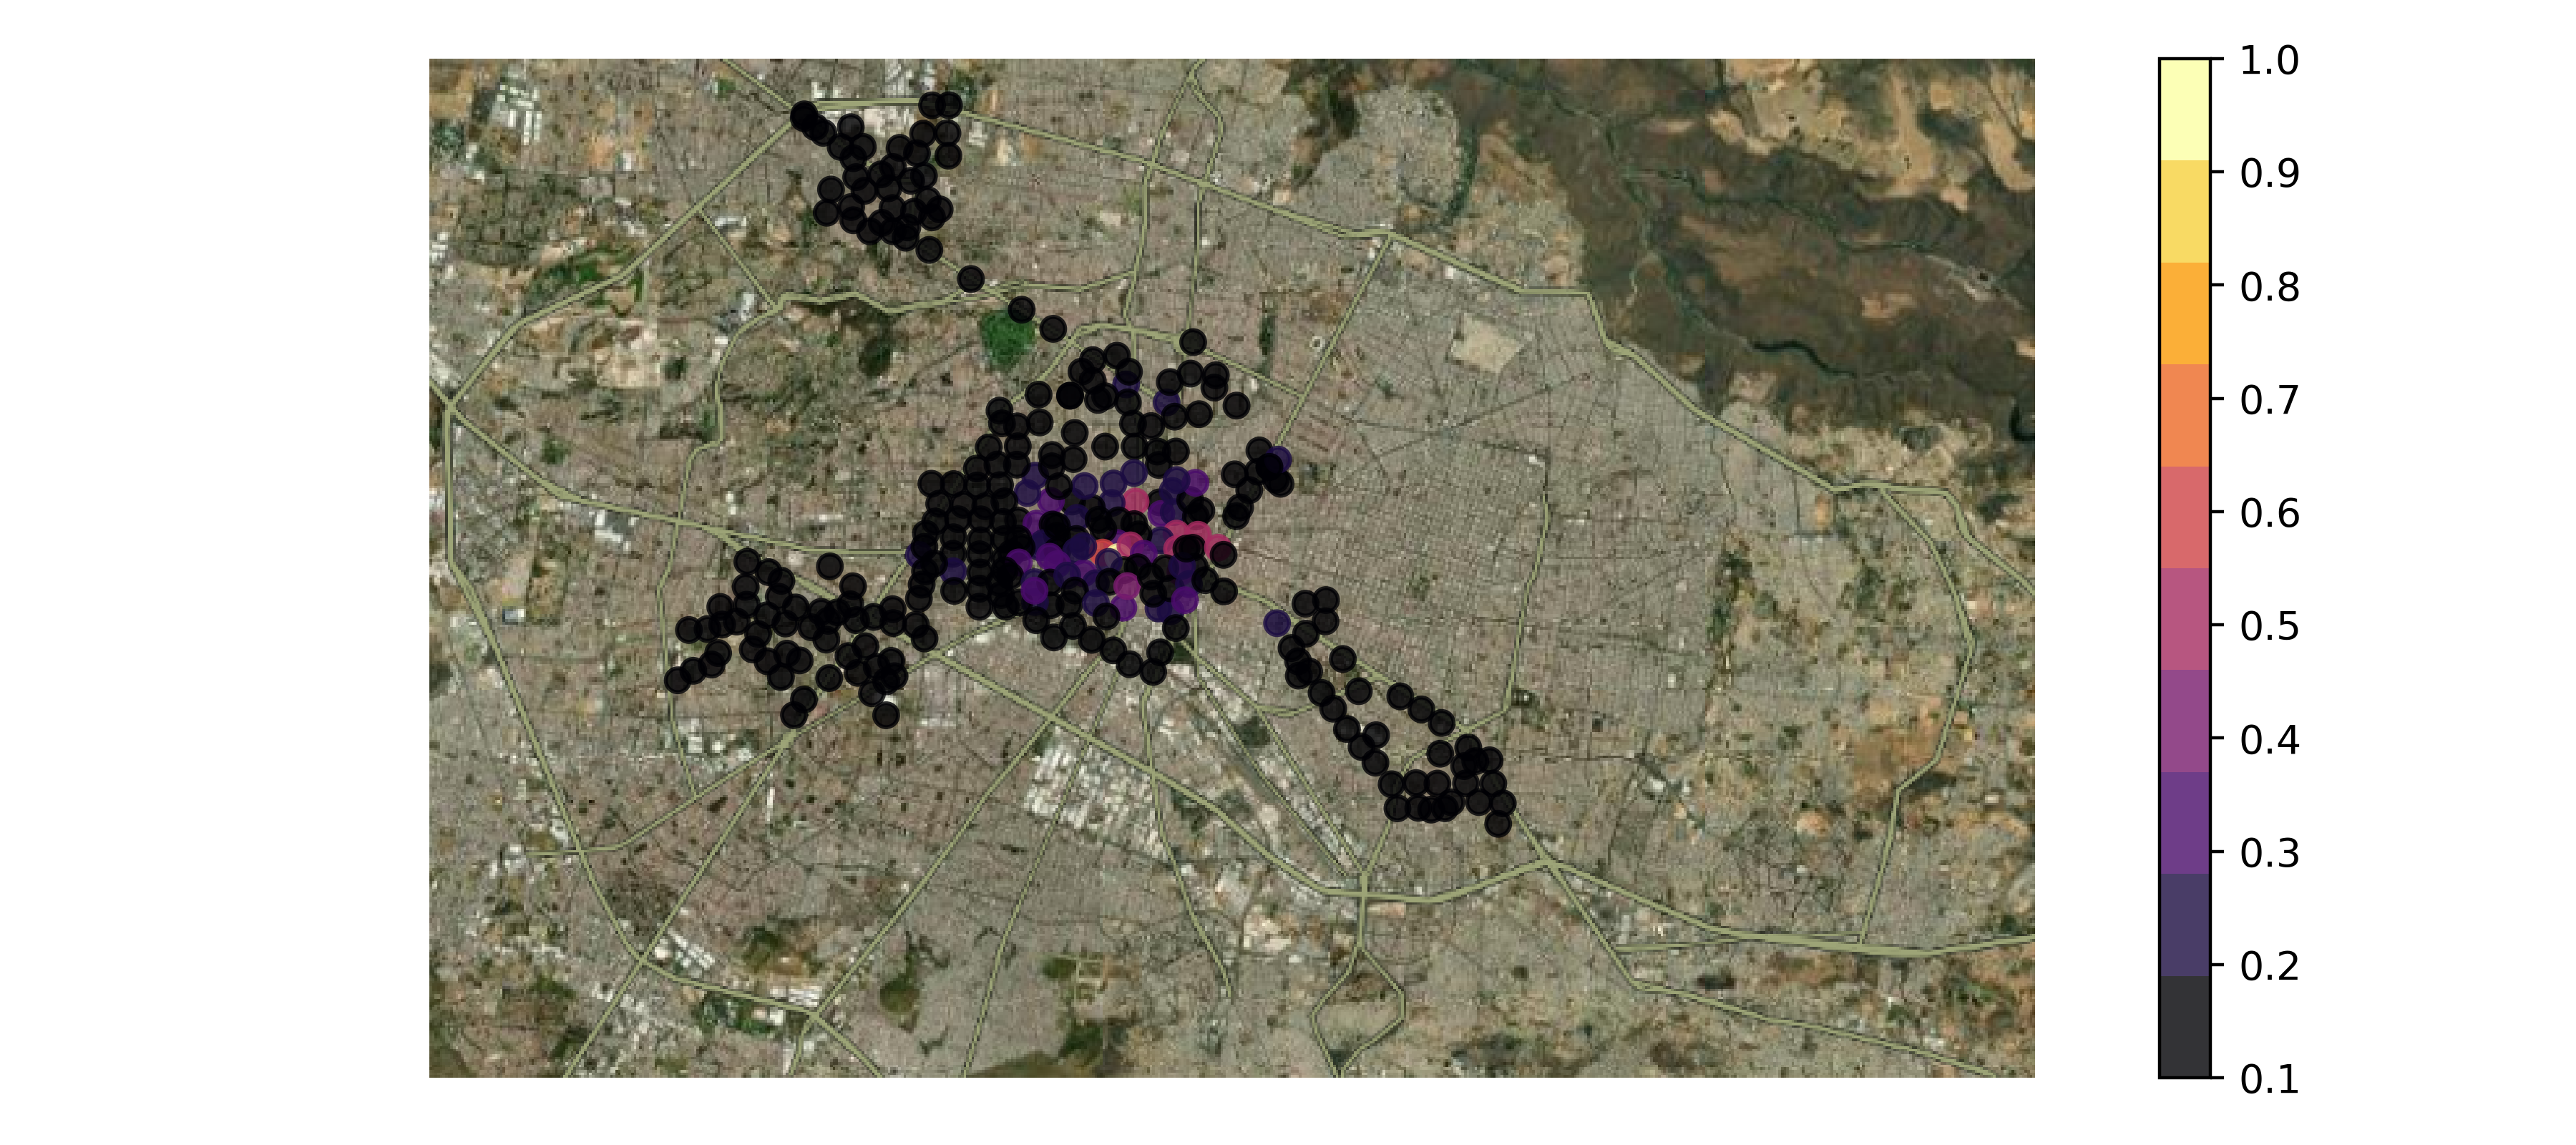
\includegraphics[width=8cm]{Graphics/repetition_destino.png}
        \caption{Zona metropolitana de Guadalajara.}
        \label{fig:distribution_station_all_destiny}
    \end{subfigure}
    \hspace{0.5cm}
    \begin{subfigure}[b]{8cm}
        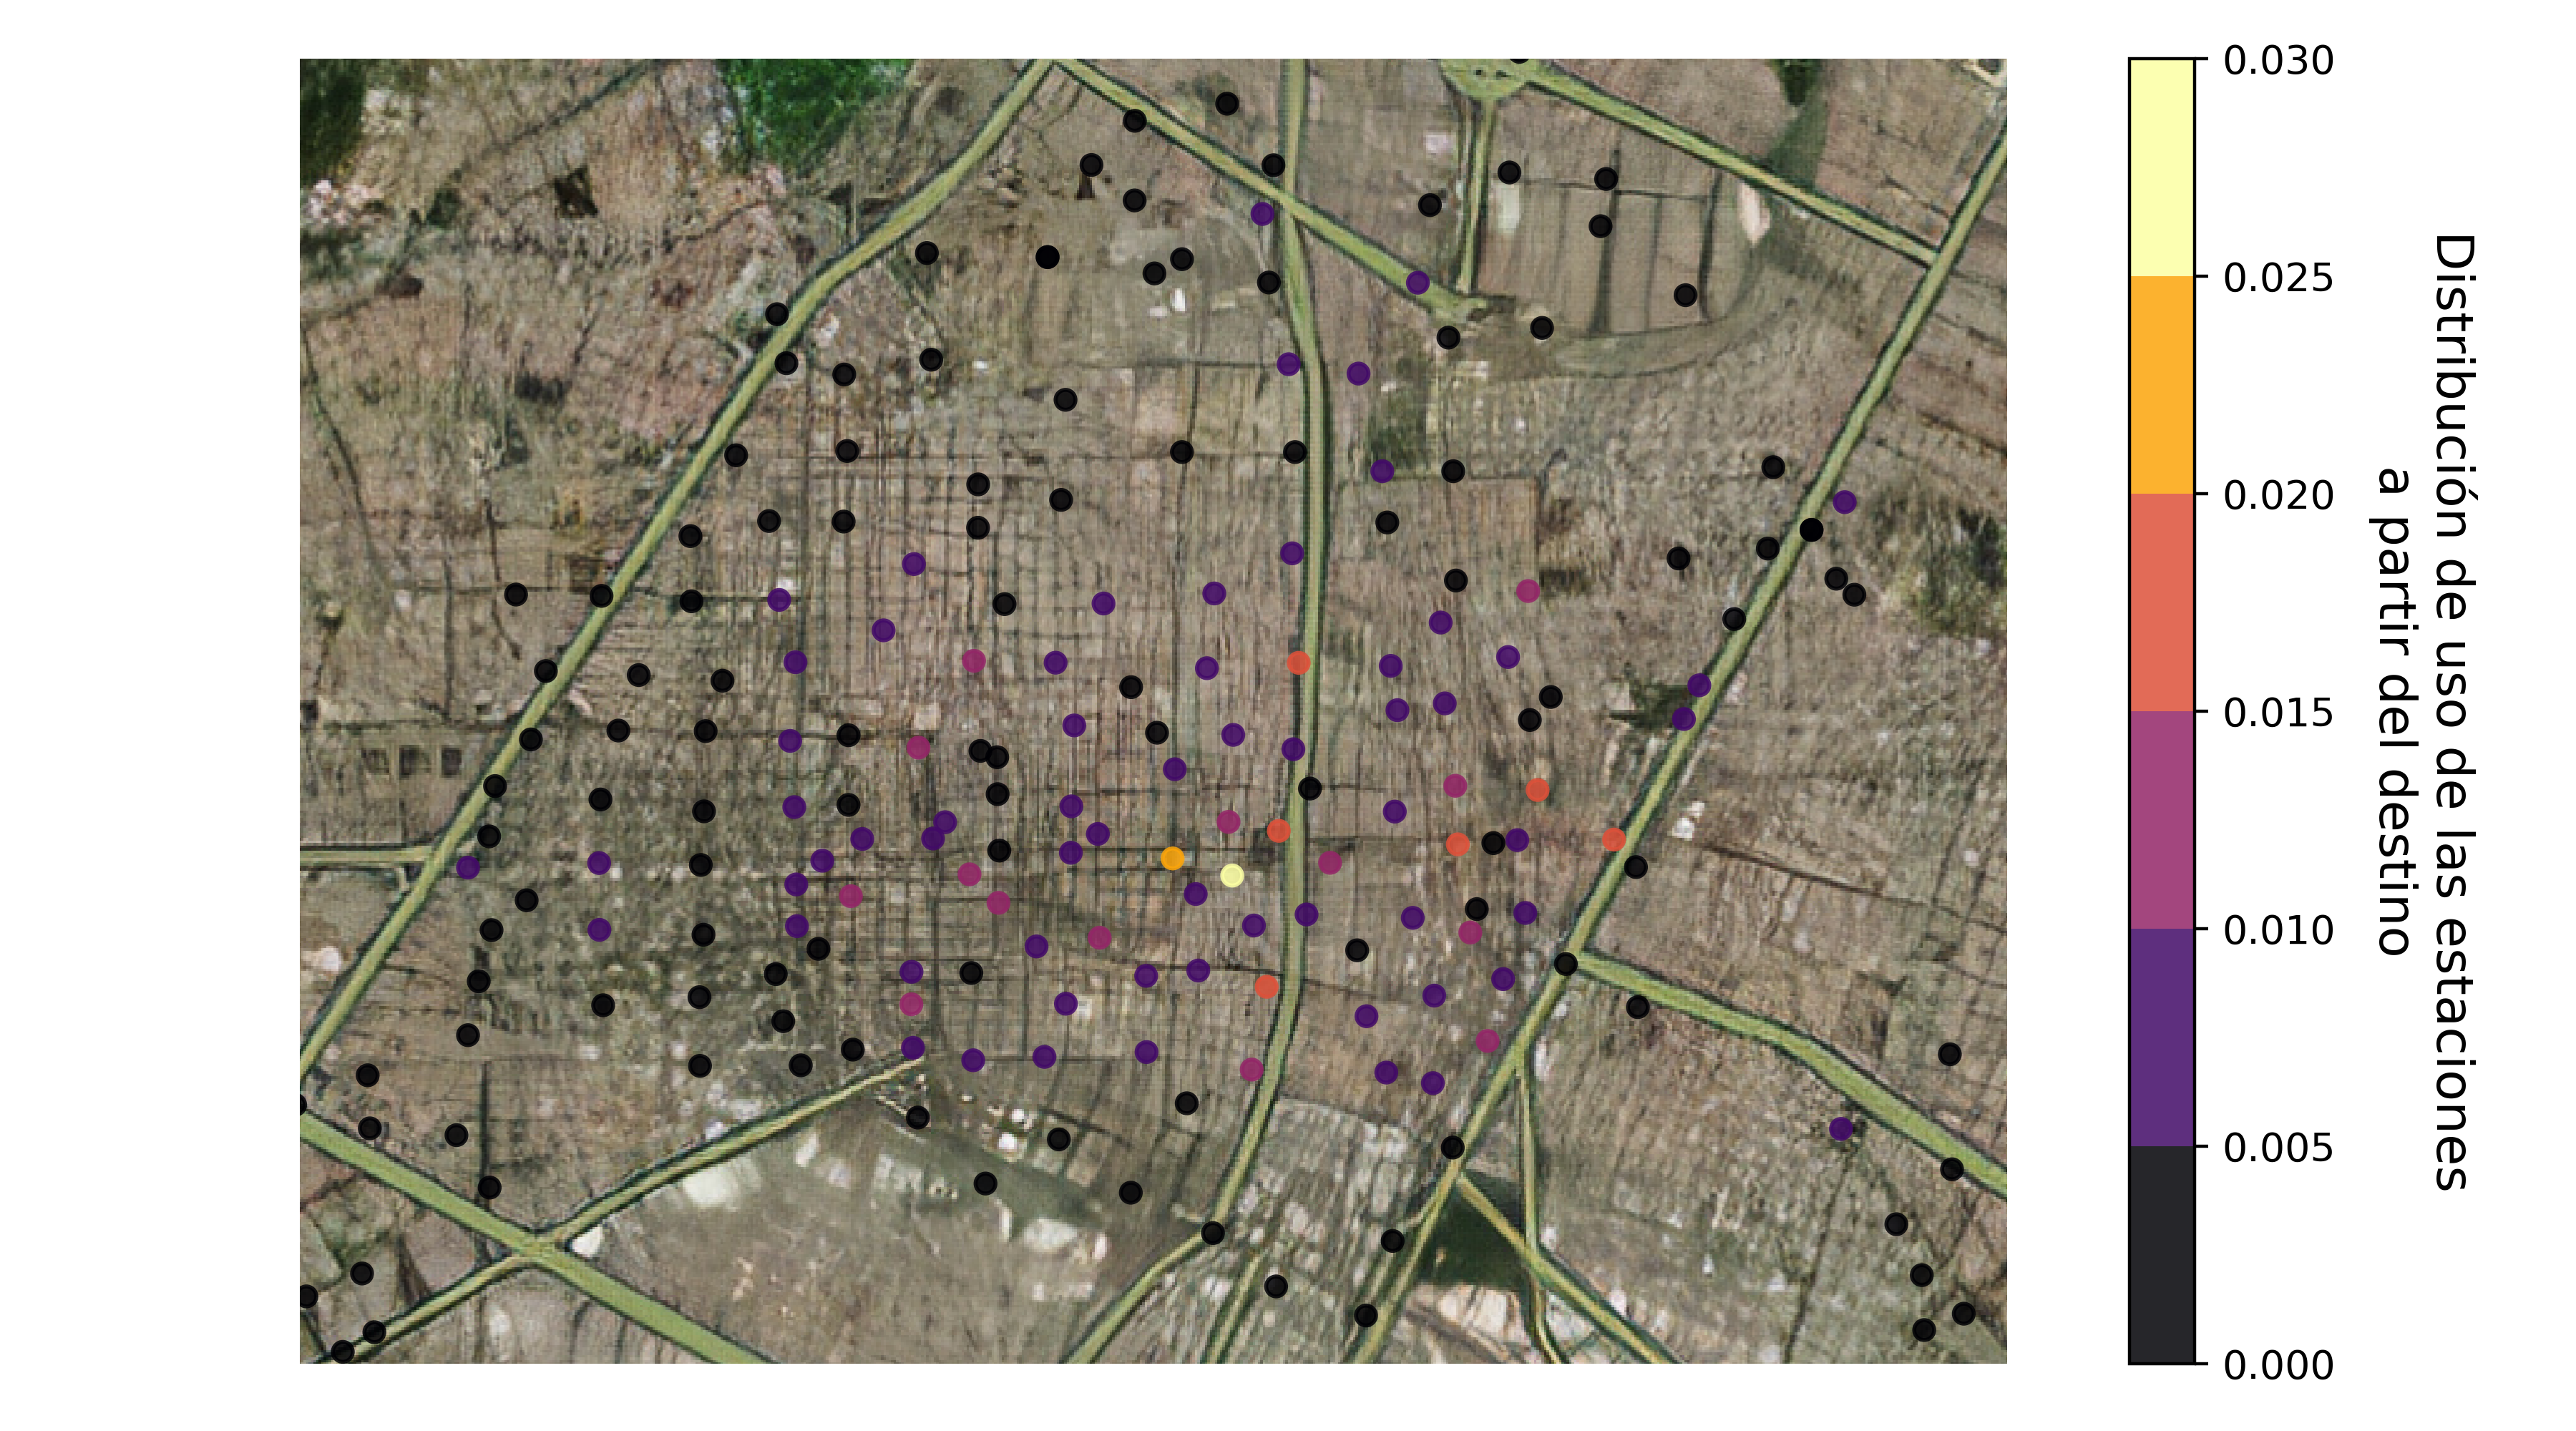
\includegraphics[width=8cm]{Graphics/repetition_destino_zoom.png}
        \caption{Zona de Chapultepec y Santa Tere.}
        \label{fig:distribution_station_zoom_destiny}
    \end{subfigure}
    \caption{Distribución del uso de las estaciones de MiBici como punto de destino.}
    \label{fig:distribution_destiny}
\end{figure}

